\section{Validation de la simulation}
La simulation d'une hiérarchie de caches étant un problème relativement compliqué, il convient de valider le fonctionnement du logiciel par différentes études des statistiques produites.

\subsection{Tests unitaires}

Quelques tests unitaires basiques ont été mis en place afin de valider les bases du logiciel. Ces tests portent notamment sur la création du fichier décrivant l'architecture à partir d'un fichier xml généré par hwloc. Ils permettent également de s'assurer de la justesse des politiques de cohérence et de remplacement pour un petit ensemble de données. En vérifiant le remplissage et les évictions de données, de même que les flags utiles aux protocoles de cohérence, quelques problèmes sont déjà levés.

\subsection{Validation comparative}

Les tests unitaires sont assez limités au sens où la validation complète du logiciel impose d'étudier l'ensemble des cas pouvant se produire sur un ensemble assez conséquent de données. Connaître précisement les résultats après $n$ opérations en déroulant soi-même l'execution de ces instructions est délicat. Il a donc fallut se tourner vers d'autres moyens de vérification. \\

Dans un premier temps, le logiciel PAPI (Performance Application Programming Interface), permettant d'utiliser les compteurs hardware d'une machine données, a été utilisé. Ce logiciel permet d'exploiter les compteurs hardware natifs présents dans les processeurs actuels. Nous avons donc utilisé ces compteurs, afin de comparer nos résultats avec les résultats obtenus sur différentes architectures. \\

Le problème posé ici est que les caches ne constituent pas l'unique réponse par rapport au problème de l'accès à la mémoire principale. En effet, un autre phénomène, le prefetching, est mis en place, et il permet notamment d'éviter les compulsory misses, c'est-à-dire les misses qui interviennent au moment où l'on charge les données dans les caches. Par exemple, lors du chargement d'un tableau, le prefetching permet de détecter qu'on est en train de charger progressivement une zone mémoire contigue, et précharge donc les données à un emplacement proche des caches. L'accès n'est alors plus compté comme un miss. \\

La validation comparative s'est donc révelée être un échec, les écarts entre notre simulation et les compteurs hardware étant théoriquement trop grande pour conclure objectivement quant aux statistiques obtenues. Par ailleurs, l'étude d'autres simulateurs de caches s'est également révelée infructueuse. Par exemple, un module du logiciel valgrind, nommé cachegrind, permet de donner les pourcentages de hits et de misses pour l'execution d'un programme. Malheureusement, leur émulation ne simule pas un comportement multi-threadés, et il a encore été impossible de conclure.
 
\subsection{Benchmarks}
La validation de notre outil a donc été possible en étudiant des codes connus pour être plus ou moins bons d'un point de vue des caches. L'étude porte sur une architecture de type \textsf{Intel} i3, i5 ou i7. Il y a $4$ caches L1, $2$ caches L2 exclusifs et $1$ L3 inclusif. La fonction ``par'' réalise des écritures sur un tableau en le partageant correctement entre les différents c{\oe}urs. La fonction ``falsesharing'' réalise une opération semblable, mais des lignes de cache sont utilisées simultanément par plusieurs c{\oe}urs. Avec la fonction ``broadcast'', tous les threads accèdent aux données du premier et avec la fonction ``pipeline'', il y a également des échanges entre les caches. Les graphiques suivants résument les statistiques basiques pour chaque niveau de cache, en faisant un moyenne lorsqu'il y a plusieurs caches pour un seul niveau.\\

\begin{figure}[l]
   \begin{minipage}[l]{.46\textwidth}
     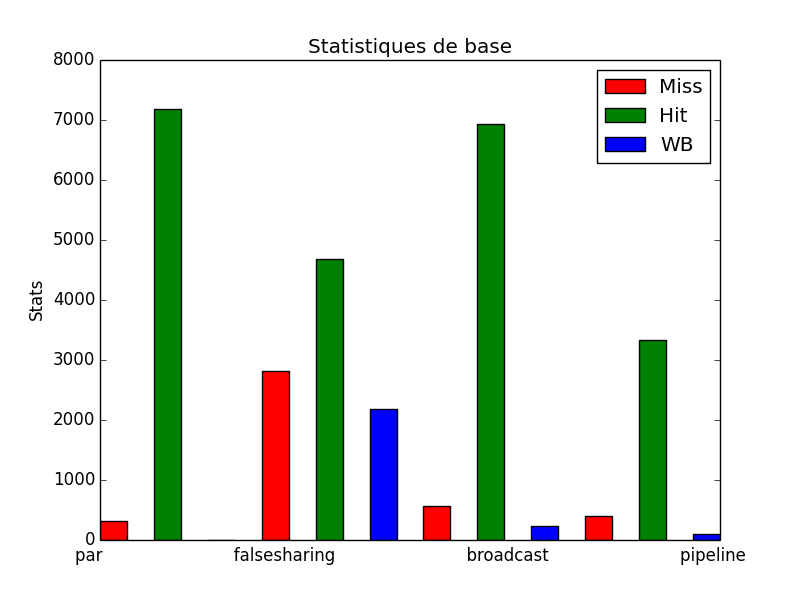
\includegraphics[scale=0.40]{images/stats_L1.png}
     \caption{\label{img:inclusifs} Statistiques pour les L1 avec des problèmes connus}
   \end{minipage} \hfill
   \begin{minipage}[r]{.46\textwidth}
     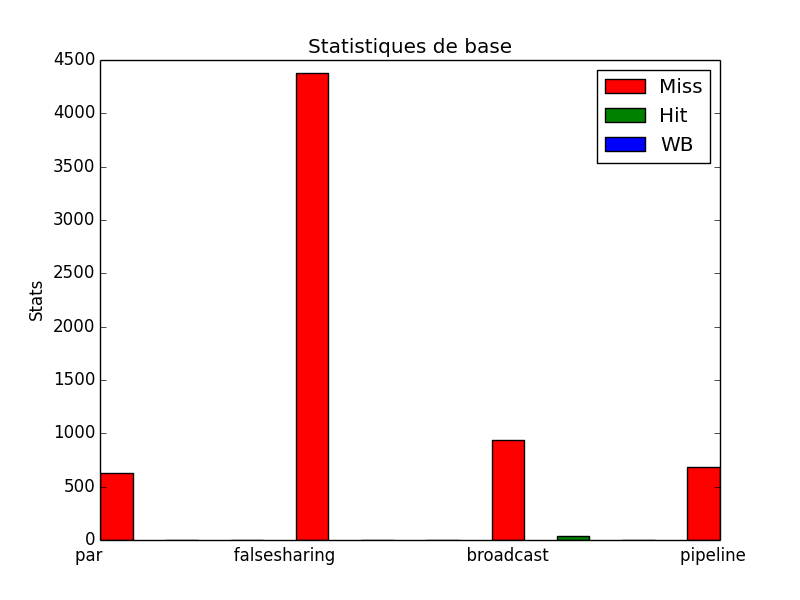
\includegraphics[scale=0.40]{images/stats_L2.png}
     \caption{\label{img:inclusifs} Statistiques pour les L2 avec des problèmes connus}
   \end{minipage}
\end{figure}

\begin{figure}[!h]
\begin{center}
   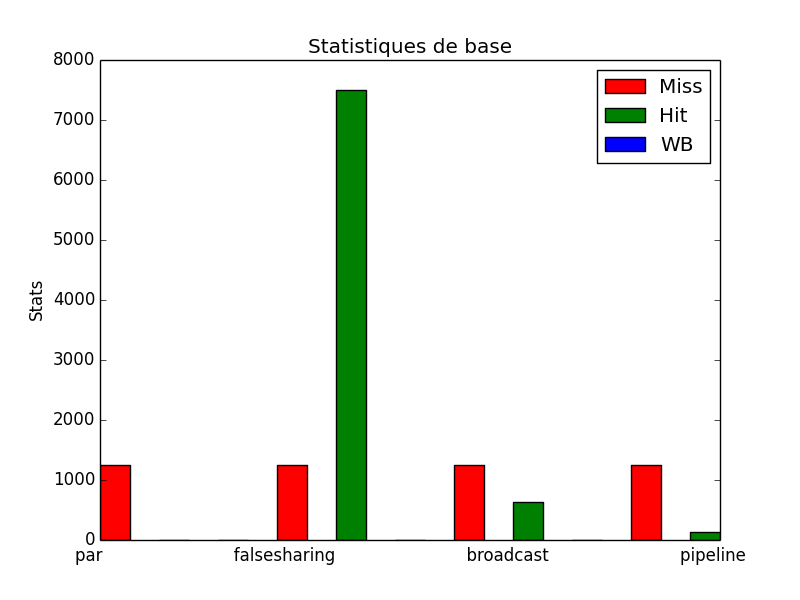
\includegraphics[scale=0.40]{images/stats_L3.png}
   \caption{\label{img:inclusifs} Statistiques pour les L3 avec des problèmes connus}
\end{center}
\end{figure}


Par ailleurs, une petite étude afin de prouver que les performances du logiciel sont bien linéaire en fonction du temps est présentée figure \ref{img:inclusifs}. \\

\begin{figure}[!h]
\begin{center}
   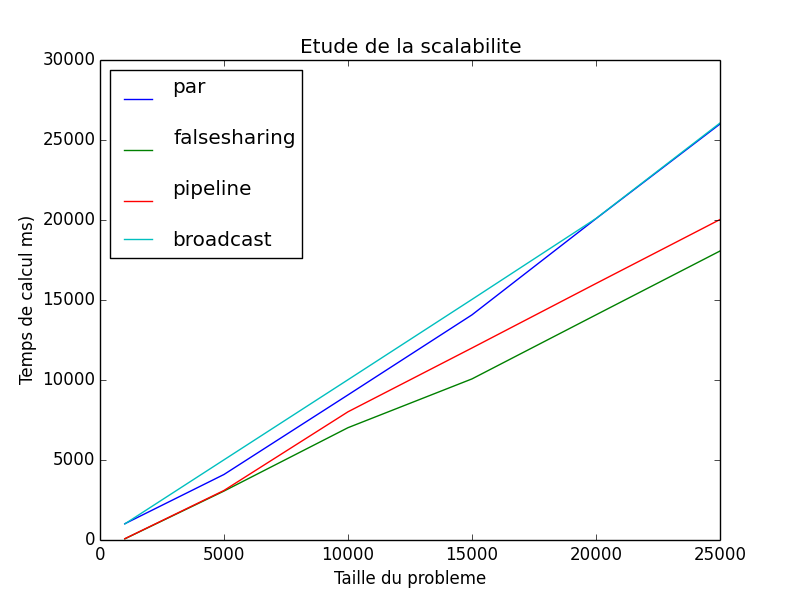
\includegraphics[scale=0.40]{images/scalability.png}
   \caption{\label{img:inclusifs} Etude de la scalabilite du programme}
\end{center}
\end{figure}
